The logged in user will have certain privileges over and above those of the base and guest users. There are two types of logged in users, namely students and lecturers who would log into the system using some form of user-name and password. The typical logged in user will be able to do the following:

\begin{figure}[h] 
  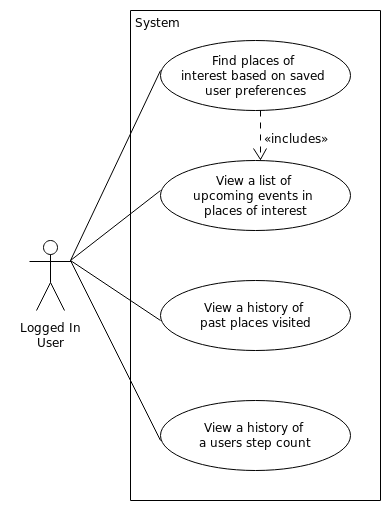
\includegraphics[width=\textwidth]{diagrams/Specific_Requirements/Loggedin_User_Case_Diagram.png}
\end{figure}

\FuncReq
{Find places of interest based on saved user preferences.}
{The users will be given the option to populate a list of preferred preferences and places of interest. The system will then generate and display a list, when needed, of the  places of interest and various events that are happening currently. This list that is provided to the user is unique and tailored to them.}
{User needs to be logged in.}
{Trivial}
\\
    \textbf{Actor system interaction model: Find places of interest based on saved user preferences. }\\
    \begin{tabular}{ | p{6cm} | p{6cm} |}
    \hline
    Actor: Logged In User & System: NavUp \\ \hline
    & 0. The system gathers all information on the logged in user.\\ \hline
    1. The user opens prefrences on points of interests. & 2. The mobile application will display various points of interest.\\ \hline
    3. The user selects various prefrences. & 4. The system updates the user's data on prefrences. \\ \hline
    & 5. The mobile application generates and displays a list of places of interest. \\ \hline
    \end{tabular}
\\
\bigskip

\FuncReq
{View a list of upcoming events in places of interest.}
{Using the saved list of preferences and places of interest that the user has provided, the system will automatically generate a list of the upcoming events that are taking place at these places and the user will be able to view them in a time-line manner and set reminders for these events.}
{User needs to be logged in.}
{Trivial}
\\
    \textbf{Actor system interaction model: View a list of upcoming events in places of interest. }\\
    \begin{tabular}{ | p{6cm} | p{6cm} |}
    \hline
    Actor: Logged In User & System: NavUp \\ \hline
    0. The user opens upcoming events and activities. & 1. The mobile application will display various upcoming events and activities.\\ \hline
    3. The user sets reminders to preferred events and activities. & 4. The system saves the reminders in the database. \\ \hline
    & 5. The mobile application notifies the user when an event is happening at appropriate times. \\ \hline
    \end{tabular}
\\
\bigskip

\FuncReq
{View a history of past places visited.}
{Users will be able to view a history of the past events that they have attended. This will include the type of event that took place and the location that the event was at.}
{User needs to be logged in.}
{Trivial}
\\
    \textbf{AView a history of past places visited. }\\
    \begin{tabular}{ | p{6cm} | p{6cm} |}
    \hline
    Actor: Logged In User & System: NavUp \\ \hline
    0. The user opens their history. & 1. The mobile application will display various locations and events the user has attended/visited.\\ \hline
    \end{tabular}
\\
\bigskip

\FuncReq
{View a history of a users step count.}
{The system will will track and record the step-count of each user, this history will be viewable by the user according to the time-line that the user will be able to specify.}
{User needs to be logged in.}
{Trivial}
\\
    \textbf{Actor system interaction model: View a history of a users step count. }\\
    \begin{tabular}{ | p{6cm} | p{6cm} |}
    \hline
    Actor: Logged In User & System: NavUp \\ \hline
    0. The user opens their profile/user information. & 1. The mobile application will display statistics of the user's step count.\\ \hline
    3. The user adjusts the timeline to view the amount of steps taken. & 4. The mobile application updates the information accordingly. \\ \hline
    \end{tabular}
\\
\bigskip
